% Slide deck for the XAI laboratory course project.
% Executive summary of report/relazione.md — every number here is copied from
% that report's generated tables. Build with `just slides` (pdflatex x2).
\documentclass[10pt,aspectratio=169]{beamer}

\usetheme{metropolis}
\metroset{sectionpage=none, numbering=fraction, progressbar=frametitle}

\usepackage[utf8]{inputenc}
\usepackage[T1]{fontenc}
\usepackage{booktabs}
\usepackage{amsmath, amssymb}
\usepackage{tikz}
\usetikzlibrary{arrows.meta, positioning, shapes.geometric, fit, backgrounds}

% Palette of the RDF/LPG figure, reused across the deck.
\definecolor{kgblue}{HTML}{3498DB}
\definecolor{kgpurple}{HTML}{9B59B6}
\definecolor{kgred}{HTML}{E74C3C}
\definecolor{kggreen}{HTML}{2ECC71}
\definecolor{kgnavy}{HTML}{2C3E50}
\definecolor{kggrey}{HTML}{7F8C8D}

\setbeamercolor{alerted text}{fg=kgred}

\newcommand{\Xmat}{\mathbf{X}}

\title{GraphLIME on RDF Knowledge Graphs}
\subtitle{Explaining R-GCN entity classification in the vocabulary of the graph}
\author{XAI Laboratory Course --- Project Report}
\date{}

\begin{document}

\maketitle

\begin{frame}{Outline}
  \setbeamertemplate{section in toc}[sections numbered]
  \tableofcontents[hideallsubsections]
\end{frame}

% ============================================================ THE PROBLEM
\section{The problem}

\begin{frame}{Motivation: an R-GCN is opaque twice over}
  Relational Graph Convolutional Networks are the standard baseline for
  entity classification on RDF knowledge graphs. They are unreadable at two
  distinct levels:

  \begin{enumerate}
    \item \textbf{As a GNN.} The decision is buried in message passing.
    \item \textbf{As an RDF model.} Its usual input is a \alert{one-hot
      entity id}, so even a perfect feature-attribution method could only
      report \emph{``entity \#4211 mattered''}.
    \end{enumerate}

  \vfill
  \begin{block}{The question of this project}
    Can we make the explanation \emph{speak RDF}? An explanation for
    ``person X belongs to research group Y'' should read \emph{``because X
    carries \texttt{swrc:publication} edges toward papers of that group''}
    --- predicates and terms of the graph, not tensor indices.
  \end{block}
\end{frame}

\begin{frame}{Why the data model matters: RDF vs.\ Labeled Property Graph}
  \centering
  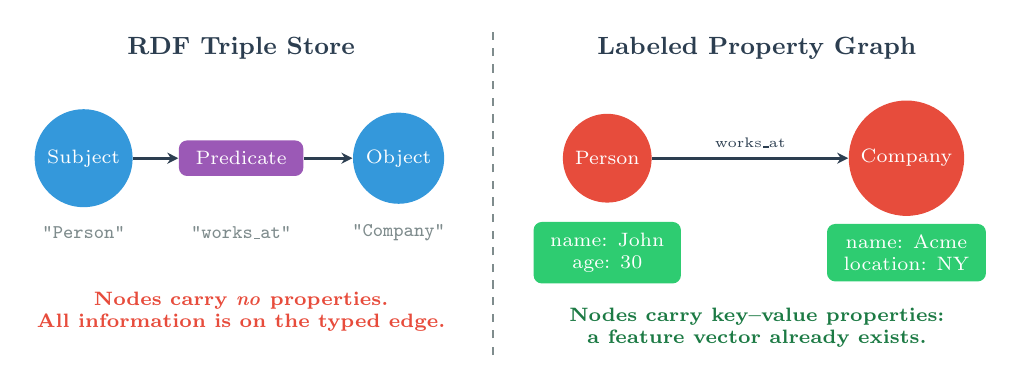
\begin{tikzpicture}[
      font=\scriptsize,
      ent/.style={circle, draw=none, text=white, minimum size=1.05cm, align=center},
      pred/.style={rounded corners=3pt, fill=kgpurple, text=white,
                   inner xsep=6pt, inner ysep=4pt},
      prop/.style={rounded corners=3pt, fill=kggreen, text=white,
                   inner xsep=6pt, inner ysep=4pt, align=center},
      ar/.style={-{Stealth[length=4pt,width=4pt]}, kgnavy, line width=1pt},
    ]

    % ---------------- left: RDF triple
    \node[kgnavy, font=\small\bfseries] at (2.35,2.0) {RDF Triple Store};
    \node[ent, fill=kgblue] (s) at (0.35,0.6) {Subject};
    \node[pred]             (p) at (2.35,0.6) {Predicate};
    \node[ent, fill=kgblue] (o) at (4.35,0.6) {Object};
    \draw[ar] (s) -- (p);
    \draw[ar] (p) -- (o);
    \node[kggrey] at (0.35,-0.35) {\texttt{"Person"}};
    \node[kggrey] at (2.35,-0.35) {\texttt{"works\_at"}};
    \node[kggrey] at (4.35,-0.35) {\texttt{"Company"}};
    \node[kgred, font=\scriptsize\bfseries, align=center] at (2.35,-1.35)
      {Nodes carry \emph{no} properties.\\All information is on the typed edge.};

    % ---------------- divider
    \draw[kggrey, dashed, line width=0.8pt] (5.55,-1.9) -- (5.55,2.2);

    % ---------------- right: labeled property graph
    \node[kgnavy, font=\small\bfseries] at (8.9,2.0) {Labeled Property Graph};
    \node[ent, fill=kgred] (a) at (7.0,0.6) {Person};
    \node[ent, fill=kgred] (b) at (10.8,0.6) {Company};
    \draw[ar] (a) -- node[above, kgnavy, font=\tiny] {works\_at} (b);
    \node[prop] (pa) at (7.0,-0.6) {name: John\\age: 30};
    \node[prop] (pb) at (10.8,-0.6) {name: Acme\\location: NY};
    \node[kggreen!60!black, font=\scriptsize\bfseries, align=center] at (8.9,-1.55)
      {Nodes carry key--value properties:\\a feature vector already exists.};
  \end{tikzpicture}

  \vfill
  \footnotesize
  Feature-attribution explainers silently assume the \emph{right-hand} model.
  RDF is the left-hand one.
\end{frame}

\begin{frame}{The crux: GraphLIME cannot be applied to RDF as published}
  GraphLIME's entire mechanism operates on a node \alert{feature matrix}: it
  collects the feature vectors of the target's neighbours and asks, via
  kernels, which \emph{feature dimensions} the model's outputs depend on.

  \vfill
  \begin{columns}[T,onlytextwidth]
    \begin{column}{0.48\textwidth}
      \textbf{Designed for citation networks}
      \begin{itemize}
        \item every node has a bag-of-words vector;
        \item every dimension \emph{is} a word --- readable by construction.
      \end{itemize}
    \end{column}
    \begin{column}{0.48\textwidth}
      \textbf{In the RDF setting}
      \begin{itemize}
        \item entities have \emph{no feature vectors at all};
        \item the one-hot entity id offers no dimension a human could read.
      \end{itemize}
    \end{column}
  \end{columns}

  \vfill
  \begin{alertblock}{Consequence}
    With no feature matrix there is nothing for HSIC Lasso to select from;
    with anonymous embedding dimensions any selection would be unreadable
    anyway. The explainer is not merely weakened --- \textbf{its input is
    undefined.} Defining that input \emph{is} the project.
  \end{alertblock}
\end{frame}

% ============================================================ THE DESIGN
\section{The proposed design}

\begin{frame}{Manufacturing the missing feature space}
  We build the feature space \alert{from the graph itself}, in the graph's
  own vocabulary --- the methodological contribution of this project.

  \vfill
  \begin{columns}[T,onlytextwidth]
    \begin{column}{0.48\textwidth}
      \begin{block}{Space A --- predicate counts}
        \texttt{out:<p>} counts the node's outgoing \texttt{<p>} edges,
        \texttt{in:<p>} its incoming ones.
        \medskip

        Coarse, dense, stable. $\approx 90$ columns on AIFB.
      \end{block}
    \end{column}
    \begin{column}{0.48\textwidth}
      \begin{block}{Space B --- predicate--object pairs}
        \texttt{out:<p>=<o>} marks having \texttt{<p>} toward the
        \emph{specific} term \texttt{<o>}.
        \medskip

        Expressive but high-dimensional and sparse, which starves the kernel
        estimates; pruned by a minimum-support threshold.
      \end{block}
    \end{column}
  \end{columns}

  \vfill
  Comparing A against B is itself one of the reported experiments.
\end{frame}

\begin{frame}{The decisive move: one shared vocabulary}
  \begin{center}
  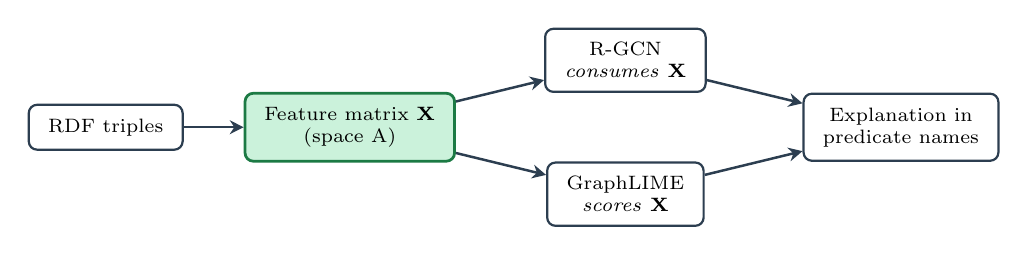
\begin{tikzpicture}[
      font=\scriptsize,
      box/.style={rounded corners=3pt, draw=kgnavy, line width=0.8pt,
                  inner xsep=7pt, inner ysep=5pt, align=center},
      hl/.style={rounded corners=3pt, fill=kggreen!25, draw=kggreen!60!black,
                 line width=1pt, inner xsep=7pt, inner ysep=5pt, align=center},
      ar/.style={-{Stealth[length=5pt,width=5pt]}, kgnavy, line width=0.9pt},
    ]
    \node[box] (rdf) at (0,0) {RDF triples};
    \node[hl]  (x)   at (3.1,0) {Feature matrix $\Xmat$\\(space A)};
    \node[box] (m)   at (6.6,0.85) {R-GCN\\\emph{consumes} $\Xmat$};
    \node[box] (e)   at (6.6,-0.85) {GraphLIME\\\emph{scores} $\Xmat$};
    \node[box] (out) at (10.1,0) {Explanation in\\predicate names};

    \draw[ar] (rdf) -- (x);
    \draw[ar] (x) -- (m);
    \draw[ar] (x) -- (e);
    \draw[ar] (m) -- (out);
    \draw[ar] (e) -- (out);
  \end{tikzpicture}
  \end{center}

  The R-GCN consumes space A \alert{in place of} the one-hot input. Model and
  explainer therefore share one vocabulary, which buys two things:

  \begin{enumerate}
    \item every feature the explainer scores is a readable statement about
      the graph (``has \texttt{publication} edges'', ``is \texttt{author}
      of \dots'');
    \item \textbf{fidelity becomes well-defined} --- otherwise undefined,
      since the explainer's features would not be what the model consumes ---
      as masking feature columns of the actual model input.
  \end{enumerate}
\end{frame}

% ============================================================ METHOD
\section{Method}

\begin{frame}{The model: R-GCN}
  Graph convolution extended to multi-relational graphs by giving every
  relation its own transformation:
  \[
    h_i^{(l+1)} = \sigma\!\Bigg( \sum_{r \in \mathcal{R}}
    \sum_{j \in \mathcal{N}_i^r} \frac{1}{c_{i,r}}\, W_r^{(l)} h_j^{(l)}
    \;+\; W_0^{(l)} h_i^{(l)} \Bigg)
  \]
  with $\mathcal{N}_i^r$ the neighbours reached through relation $r$,
  $c_{i,r}=|\mathcal{N}_i^r|$, and $W_0$ a self-loop term.

  \vfill
  \textbf{Why per-relation weights.} In a knowledge graph the meaning lives
  in the edge \emph{types}; a plain GCN would collapse \texttt{author} and
  \texttt{employs} into an undifferentiated ``neighbour''.

  \textbf{Basis decomposition.} One matrix per relation is prohibitive
  (45 relations on AIFB), so
  $W_r^{(l)} = \sum_{b=1}^{B} a_{rb}^{(l)} V_b^{(l)}$ --- parameter sharing
  that doubles as regularisation.
\end{frame}

\begin{frame}{HSIC: measuring non-linear dependence}
  The Hilbert--Schmidt Independence Criterion is a kernel measure of
  statistical dependence. With kernel matrices $K$, $L$ and centering matrix
  $H = I - \tfrac{1}{n}\mathbf{1}\mathbf{1}^{\!\top}$:
  \[
    \widehat{\mathrm{HSIC}}(K,L) \;=\; \frac{\operatorname{tr}(KHLH)}{(n-1)^2}
  \]

  For characteristic kernels (RBF, median-heuristic bandwidth) it vanishes
  exactly when the variables are independent.

  \vfill
  \begin{block}{Why kernels and not a linear surrogate}
    $y = x^2$ with $x$ symmetric around zero has Pearson correlation
    $\approx 0$ but clearly positive HSIC. A GNN's output is a non-linear
    function of its input, so a linear surrogate would measure the wrong
    thing. Our property tests assert this explicitly.
  \end{block}
\end{frame}

\begin{frame}{HSIC Lasso and its three-term reading}
  With centered, Frobenius-normalised kernels $\bar K_k$ (features) and
  $\bar L$ (model output), solve the non-negative Lasso
  \[
    \min_{\beta \ge 0} \;\; \tfrac{1}{2}
    \Big\| \bar L - \sum\nolimits_{k=1}^{d} \beta_k \bar K_k \Big\|_F^2
    + \rho \|\beta\|_1 .
  \]
  Expanding the square exposes the \alert{explainable three-term form}:
  \[
    \min_{\beta \ge 0} \;\;
    \underbrace{-\sum_k \beta_k \mathrm{HSIC}(x_k, y)}_{\textbf{relevance}}
    \;+\;
    \underbrace{\tfrac{1}{2}\sum_{k,l}\beta_k\beta_l \mathrm{HSIC}(x_k,x_l)}_{\textbf{redundancy}}
    \;+\;
    \underbrace{\rho\|\beta\|_1}_{\textbf{sparsity}}
  \]

  \vfill
  Term 1 rewards features the output depends on; term 2 penalises features
  redundant with one another; term 3 forces most weights to zero. The
  resulting $\beta_k \ge 0$ is feature $k$'s importance.
\end{frame}

\begin{frame}{GraphLIME}
  Unlike LIME, GraphLIME \alert{perturbs nothing}. To explain node $v$:

  \begin{itemize}
    \item the ``samples'' are the \textbf{real nodes of $v$'s $h$-hop
      neighbourhood} ($h=2$ here);
    \item $\Xmat$ collects their features, $Y$ the model's predicted
      probability vectors;
    \item HSIC Lasso on $(\Xmat, Y)$ yields a sparse $\beta$ over feature
      dimensions.
  \end{itemize}

  \vfill
  \begin{columns}[T,onlytextwidth]
    \begin{column}{0.48\textwidth}
      \begin{alertblock}{It explains features, not edges}
        On a graph whose nodes have no features the method has no input at
        all --- the situation of Section~1.
      \end{alertblock}
    \end{column}
    \begin{column}{0.48\textwidth}
      \begin{alertblock}{Its samples are a neighbourhood}
        A small neighbourhood means few samples and a meaningless HSIC
        estimate, so the pipeline \textbf{refuses} nodes below a minimum
        size rather than emit noise.
      \end{alertblock}
    \end{column}
  \end{columns}
\end{frame}

\begin{frame}{The pipeline end to end}
  \centering
  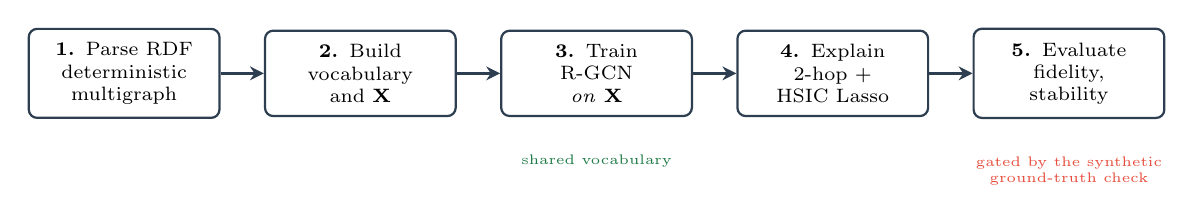
\begin{tikzpicture}[
      font=\scriptsize, node distance=0.55cm,
      st/.style={rounded corners=3pt, draw=kgnavy, line width=0.8pt,
                 inner xsep=6pt, inner ysep=5pt, align=center,
                 text width=2.0cm},
      ar/.style={-{Stealth[length=5pt,width=5pt]}, kgnavy, line width=0.9pt},
    ]
    \node[st] (a) {\textbf{1.} Parse RDF\\deterministic\\multigraph};
    \node[st, right=of a] (b) {\textbf{2.} Build\\vocabulary\\and $\Xmat$};
    \node[st, right=of b] (c) {\textbf{3.} Train R-GCN\\\emph{on} $\Xmat$};
    \node[st, right=of c] (d) {\textbf{4.} Explain\\2-hop $+$\\HSIC Lasso};
    \node[st, right=of d] (e) {\textbf{5.} Evaluate\\fidelity,\\stability};

    \draw[ar] (a) -- (b);
    \draw[ar] (b) -- (c);
    \draw[ar] (c) -- (d);
    \draw[ar] (d) -- (e);

    \node[kggreen!60!black, font=\tiny, align=center, below=0.35cm of c]
      {shared vocabulary};
    \node[kgred, font=\tiny, align=center, below=0.35cm of e]
      {gated by the synthetic\\ground-truth check};
  \end{tikzpicture}

  \vfill
  \raggedright
  \footnotesize
  Non-zero $\beta$ are mapped back to \textbf{predicate names}. HSIC and the
  solver are implemented from scratch, with property tests written
  \emph{before} the implementation: symmetry, non-negativity,
  $\mathrm{nHSIC} \in [0,1]$, joint-permutation invariance, weight-splitting
  for duplicated features, and sparsity monotone in $\rho$.
\end{frame}

\begin{frame}{Baseline: GNNExplainer}
  GNNExplainer (Ying et al., 2019) natively optimises a soft mask over
  \emph{edges} via mutual information.

  \vfill
  \begin{block}{A structural incompatibility}
    Its edge masks cannot be applied to \texttt{RGCNConv}, which runs one
    propagate per relation on edge subsets --- a full-graph mask can never
    align.
  \end{block}

  \vfill
  \textbf{Resolution.} The baseline uses GNNExplainer's \alert{attribute
  mask} over the same feature matrix: it scores exactly the features
  GraphLIME scores, making the two rankings directly comparable at the
  predicate level. The price is that the comparison covers feature
  attribution only.
\end{frame}

% ============================================================ SETUP
\section{Experimental setup}

\begin{frame}{Datasets and model}
  \begin{table}
    \footnotesize
    \begin{tabular}{lrrrl}
      \toprule
      \textbf{Dataset} & \textbf{Nodes} & \textbf{Triples} & \textbf{Predicates} & \textbf{Task} \\
      \midrule
      AIFB  &  8{,}285 & 29{,}043 & 45 & research-group affiliation (4 classes) \\
      MUTAG & 23{,}644 & 74{,}227 & 23 & mutagenicity (2 classes) \\
      \bottomrule
    \end{tabular}
  \end{table}

  \vfill
  \begin{columns}[T,onlytextwidth]
    \begin{column}{0.48\textwidth}
      \textbf{Model}
      \begin{itemize}
        \item 2-layer \texttt{RGCNConv}, 30 bases, hidden 32
        \item Adam, lr $0.01$, 200 epochs, 5 seeds
        \item predicate-count features, both directions
      \end{itemize}
    \end{column}
    \begin{column}{0.48\textwidth}
      \textbf{Explanations}
      \begin{itemize}
        \item 2-hop neighbourhoods, subsampled above 200 nodes
        \item RBF kernels, median heuristic, $\rho = 0.1$
        \item neighbourhoods under 10 nodes refused
      \end{itemize}
    \end{column}
  \end{columns}

  \vfill
  \footnotesize
  Label-revealing predicates (\texttt{employs}/\texttt{affiliation},
  \texttt{isMutagenic}) are absent from the dumps; a blocklist
  \textbf{asserts} their absence at every load.
\end{frame}

\begin{frame}{The correctness gate: synthetic ground truth}
  On real data there is no ground-truth explanation. Before \emph{any} number
  on AIFB or MUTAG was produced, the pipeline had to recover a planted rule.

  \vfill
  \begin{block}{Generated graph where class $1 \Longleftrightarrow$ the entity has predicate $p_7$}
    \begin{itemize}
      \item GraphLIME ranked \texttt{out:syn:p7} \alert{first} for
        $\ge 95\%$ of explained nodes at $0\%$ noise;
      \item it kept the target \textbf{top-3} under two distractor
        predicates $90\%$-correlated with it;
      \item $\mathrm{fid}^+ >$ random-$k$ is \emph{asserted} here.
    \end{itemize}
    It passed on the first run.
  \end{block}

  \vfill
  On real data the numbers are \textbf{reported, not asserted}: no threshold
  is ever lowered to make progress.
\end{frame}

% ============================================================ RESULTS
\section{Results}

\begin{frame}{The evaluation metrics (1/2)}
  Let $S_k$ be the top-$k$ features by $\beta$, and $f_{\hat y}$ the model's
  probability for the predicted class.

  \vfill
  \begin{block}{Fidelity$+$ --- necessity \quad \emph{(higher is better)}}
    \vspace{-1.5ex}
    \[
      \mathrm{fid}^+ = \tfrac{1}{|V|}\sum_{v\in V}
      \big[ f_{\hat y}(x_v) - f_{\hat y}(x_v^{\setminus S_k}) \big]
    \]
    \vspace{-2ex}

    Zero the top-$k$ columns: if they matter, the prediction should fall.
  \end{block}

  \begin{block}{Fidelity$-$ --- sufficiency \quad \emph{(lower is better)}}
    \vspace{-1.5ex}
    \[
      \mathrm{fid}^- = \tfrac{1}{|V|}\sum_{v\in V}
      \big[ f_{\hat y}(x_v) - f_{\hat y}(x_v^{S_k}) \big]
    \]
    \vspace{-2ex}

    Keep \emph{only} the top-$k$: if they suffice, the prediction should survive.
  \end{block}

  \vfill
  \alert{Random-$k$ control.} Masking any $k$ columns perturbs the
  prediction, so both metrics are recomputed on a random $k$-subset. The
  evidence is the \textbf{gap}, not the raw value.
\end{frame}

\begin{frame}{The evaluation metrics (2/2)}
  \begin{block}{Stability --- Jaccard@5}
    $J(S,S') = \dfrac{|S \cap S'|}{|S \cup S'|} \in [0,1]$, averaged over
    explained nodes, computed across \textbf{training seeds} and across
    \textbf{hops} $\in \{1,2,3\}$. An explainer that changes its answer when
    nothing meaningful changed is not trustworthy.
  \end{block}

  \begin{block}{Agreement --- Jaccard@5 over predicates}
    The same index after collapsing each feature to its predicate URI, used
    for \textbf{space A vs.\ space B} and \textbf{GraphLIME vs.\
    GNNExplainer}. Not a correctness measure --- there is no reference
    ranking --- so it is read as a sensitivity analysis.
  \end{block}

  \begin{block}{Refusal rate}
    Fraction of entities whose neighbourhood falls below
    \texttt{min\_neighborhood} $= 10$. A refusal is a finding about
    applicability, not a failure.
  \end{block}
\end{frame}

\begin{frame}{Classification accuracy}
  \begin{table}
    \footnotesize
    \begin{tabular}{lccc}
      \toprule
      \textbf{Dataset} & \textbf{Test accuracy (5 seeds)} & \textbf{Best seed} & \textbf{R-GCN paper (one-hot)} \\
      \midrule
      AIFB  & $0.8833 \pm 0.0534$ & $0.9444$ & $0.958$ \\
      MUTAG & $0.7559 \pm 0.0305$ & $0.7941$ & $0.732$ \\
      \bottomrule
    \end{tabular}
  \end{table}

  \vfill
  \textbf{Interpretation.} The interpretable feature space is no handicap on
  MUTAG, whose 5-seed mean \emph{exceeds} the one-hot R-GCN, while AIFB lands
  several points below its $0.958$. AIFB's classes hinge on \emph{which}
  specific entity a person is connected to --- exactly what per-entity
  embeddings encode for free and predicate counts deliberately discard.

  \vfill
  \begin{center}
    \alert{The cost of interpretability is visible, dataset-dependent, and
    paid in the input representation --- not in the explainer.}
  \end{center}
\end{frame}

\begin{frame}{Explanation fidelity: the numbers}
  \begin{table}
    \scriptsize
    \begin{tabular}{llcccc}
      \toprule
      \textbf{Dataset} & $k$ & \textbf{fidelity}$+$ & \textbf{random}$+$ & \textbf{fidelity}$-$ & \textbf{random}$-$ \\
      \midrule
      AIFB  & 1  & 0.0176 & 0.0129 & 0.7145 & 0.6767 \\
      AIFB  & 2  & 0.0162 & 0.0066 & 0.7386 & 0.7556 \\
      AIFB  & 5  & 0.1079 & 0.0520 & 0.7160 & 0.6085 \\
      AIFB  & 10 & 0.1829 & 0.0735 & 0.6338 & 0.6184 \\
      \midrule
      MUTAG & 1  & 0.0789 & $-0.0013$ & 0.5397 & 0.3151 \\
      MUTAG & 2  & 0.1224 & 0.0205 & 0.3068 & 0.2744 \\
      MUTAG & 5  & 0.1627 & 0.0475 & 0.1987 & 0.3352 \\
      MUTAG & 10 & 0.0999 & 0.1592 & 0.2299 & 0.3462 \\
      \bottomrule
    \end{tabular}
  \end{table}
  \footnotesize
  36 explained nodes on AIFB, 68 on MUTAG.

  \vfill
  \textbf{Sufficiency.} On AIFB $\mathrm{fid}^-$ stays high at every $k$
  ($\approx 0.7$): no five features \emph{suffice}, the model spreads
  evidence across the whole neighbourhood profile. On MUTAG the top-5
  preserve the prediction markedly better than random-5
  ($0.199$ vs.\ $0.335$).
\end{frame}

\begin{frame}{Fidelity$+$ vs.\ $k$ against the random-$k$ control}
  \begin{center}
    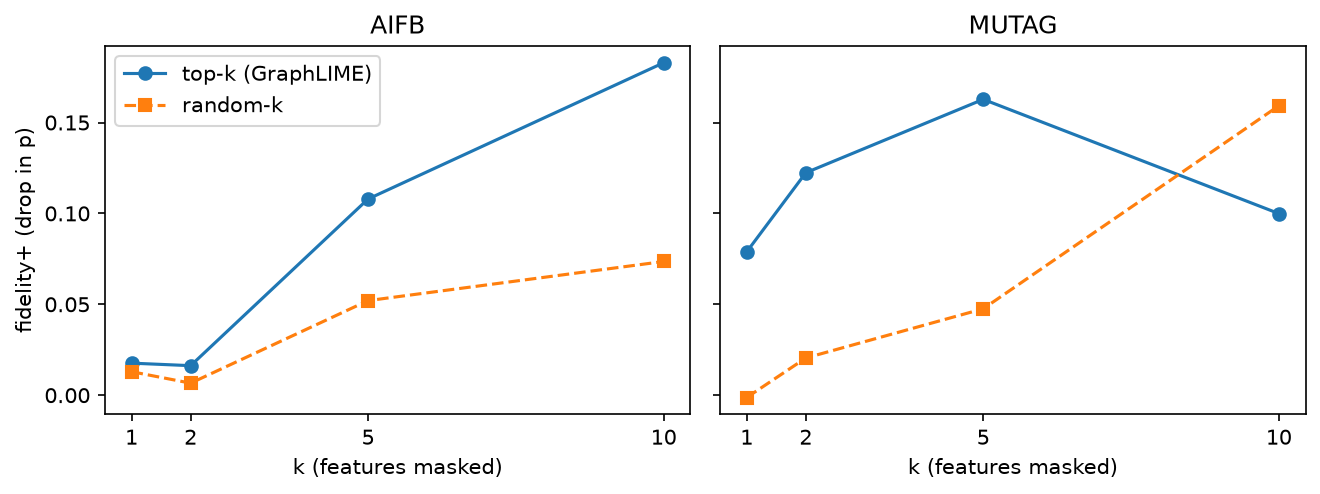
\includegraphics[width=0.86\textwidth]{../results/figures/fidelity_curve.png}
  \end{center}

  \vfill
  \textbf{Interpretation.} For $k \le 5$ the GraphLIME curve sits clearly
  above the random control on both datasets: the explanations point at
  features the model actually uses. The inversion at $k = 10$ on MUTAG
  reflects the sweep, not the method --- explanations carry fewer than ten
  non-zero $\beta$, so the top-10 set pads with irrelevant columns.
\end{frame}

\begin{frame}{Explanation stability across seeds and hops}
  \begin{center}
    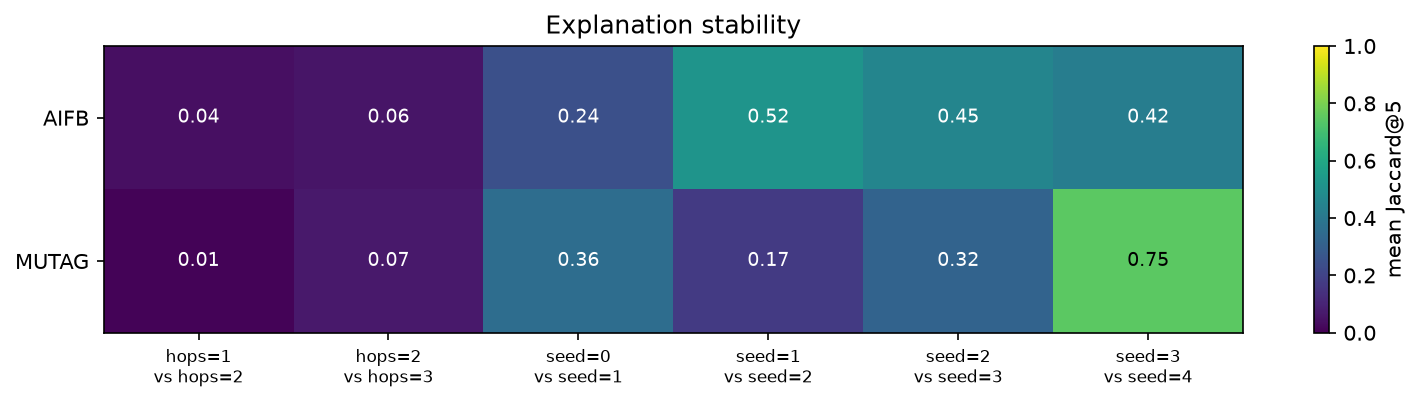
\includegraphics[width=0.94\textwidth]{../results/figures/stability_heatmap.png}
  \end{center}

  \vfill
  \textbf{Interpretation.} Across training seeds agreement is moderate
  (Jaccard@5 $0.17$--$0.75$): models of comparable accuracy use partially
  different features. Across hops it is near zero ($0.01$--$0.07$), because
  GraphLIME's samples \emph{are} the neighbourhood --- \alert{the radius is
  the single most consequential explanation hyperparameter}.
\end{frame}

\begin{frame}{Feature-space sensitivity and baseline agreement}
  \begin{columns}[c,onlytextwidth]
    \begin{column}{0.54\textwidth}
      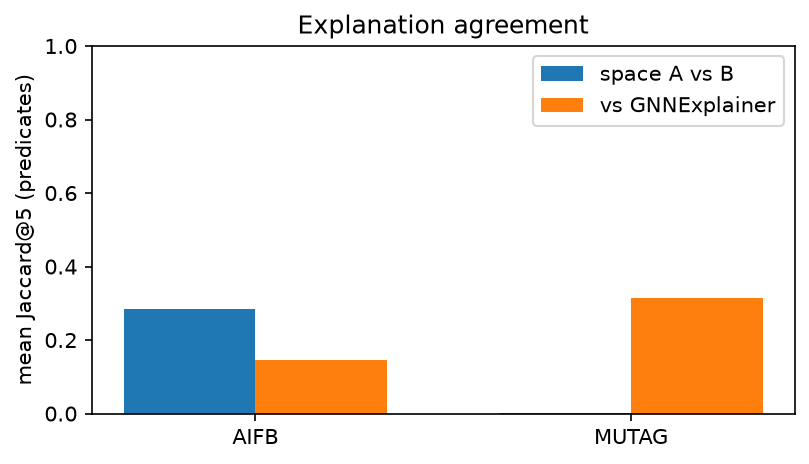
\includegraphics[width=\textwidth]{../results/figures/agreement_comparison.png}
    \end{column}
    \begin{column}{0.44\textwidth}
      \scriptsize
      \begin{tabular}{lc}
        \toprule
        \textbf{Comparison} & \textbf{Jaccard@5} \\
        \midrule
        AIFB, space A vs.\ B      & 0.2843 \\
        AIFB, vs.\ GNNExplainer   & 0.1456 \\
        MUTAG, space A vs.\ B     & 0.0029 \\
        MUTAG, vs.\ GNNExplainer  & 0.3153 \\
        \bottomrule
      \end{tabular}
    \end{column}
  \end{columns}

  \vfill
  \textbf{Interpretation.} A-vs-B overlap is moderate on AIFB and essentially
  zero on MUTAG, where space B shifts weight onto specific \texttt{rdf:type}
  objects (atom types) that space A cannot express. Agreement with
  GNNExplainer is limited on both --- kernel dependence and a learned soft
  mask answer distinct questions --- so the disagreement is itself the
  reported result.
\end{frame}

\begin{frame}{Refusals and qualitative output}
  \begin{columns}[T,onlytextwidth]
    \begin{column}{0.46\textwidth}
      \begin{table}
        \footnotesize
        \begin{tabular}{lccc}
          \toprule
          & \textbf{Expl.} & \textbf{Ref.} & \textbf{Rate} \\
          \midrule
          AIFB  & 36 & 0 & 0.0000 \\
          MUTAG & 68 & 0 & 0.0000 \\
          \bottomrule
        \end{tabular}
      \end{table}
      \footnotesize
      At 2 hops every test entity clears
      \texttt{min\_neighborhood} $=10$. The guard was never \emph{needed} at
      this radius --- not absent: it is exercised by the test suite and by
      smaller-radius runs.
    \end{column}
    \begin{column}{0.50\textwidth}
      \begin{block}{Explanations in the graph's vocabulary}
        \footnotesize
        The executed notebook prints sentence-form explanations from the
        committed checkpoints, e.g.\ a person correctly predicted into a
        research group \emph{because of} \texttt{publication} and
        \texttt{author} edges toward that group's papers, or a MUTAG bond
        classified through its atom-type context.
        \medskip

        Refusals are printed inline, not skipped.
      \end{block}
    \end{column}
  \end{columns}
\end{frame}

% ============================================================ LIMITATIONS
\section{Limitations and conclusions}

\begin{frame}{Limitations}
  \begin{itemize}
    \item \textbf{Dependence, not causation.} $\beta$ is a local,
      kernel-level account of dependence fitted on one neighbourhood; it
      does not license causal or global claims.
    \item \textbf{Fidelity on columns, not structure.} Masking a column
      removes the evidence of a predicate but leaves the edges intact;
      deleting the triples themselves would be more faithful to RDF
      semantics, at a substantially higher cost.
    \item \textbf{Neighbourhood distortions at the extremes.} Subsampled
      above 200 nodes, refused below 10 --- and in between, the radius
      dominates the outcome.
    \item \textbf{Two small benchmarks.} 176 and 340 labelled entities put
      every mean on a few tens of test nodes; conclusions are claimed at
      this scale only.
    \item \textbf{The baseline is not like-for-like.} GNNExplainer is
      compared through its attribute mask, so the comparison covers feature
      attributions, not edge attributions.
  \end{itemize}
\end{frame}

\begin{frame}{Conclusions}
  \begin{enumerate}
    \item GraphLIME cannot be applied to RDF as published: its input, a node
      feature matrix, \alert{does not exist} in a triple store.
    \item Defining that input from the graph's own predicates makes the
      method applicable \emph{and} makes its output readable by a domain
      expert --- explanations are statements about predicates, not tensor
      indices.
    \item Letting the R-GCN consume the same matrix makes \textbf{fidelity
      measurable at all}, and the cost of interpretability is then visible:
      MUTAG above the one-hot baseline, AIFB below it.
    \item The explanations beat the random control for $k \le 5$ on both
      datasets, and the pipeline recovers a planted ground-truth rule.
    \item The honest negative finding: on knowledge graphs of this size,
      \textbf{the neighbourhood radius dictates the explanation}, which
      bounds how far a single GraphLIME explanation should be trusted.
  \end{enumerate}

  \vfill
  \centering
  \footnotesize
  For the full argument, derivations and per-seed numbers, see
  \texttt{report/relazione.md}.
\end{frame}

\begin{frame}{References}
  \scriptsize
  \begin{thebibliography}{9}
    \setlength{\itemsep}{0.35em}
    \bibitem{rgcn} Schlichtkrull et al.
      \newblock \emph{Modeling Relational Data with Graph Convolutional
      Networks}. ESWC 2018.
    \bibitem{graphlime} Huang et al.
      \newblock \emph{GraphLIME: Local Interpretable Model Explanations for
      Graph Neural Networks}. 2020.
    \bibitem{hsiclasso} Yamada et al.
      \newblock \emph{High-Dimensional Feature Selection by Feature-Wise
      Kernelized Lasso}. Neural Computation, 2014.
    \bibitem{hsic} Gretton et al.
      \newblock \emph{Measuring Statistical Dependence with Hilbert-Schmidt
      Norms}. ALT 2005.
    \bibitem{gnnexplainer} Ying et al.
      \newblock \emph{GNNExplainer: Generating Explanations for Graph Neural
      Networks}. NeurIPS 2019.
  \end{thebibliography}
\end{frame}

\end{document}
